% A plane graph and its dual (generated by figs_c1ch10.py).
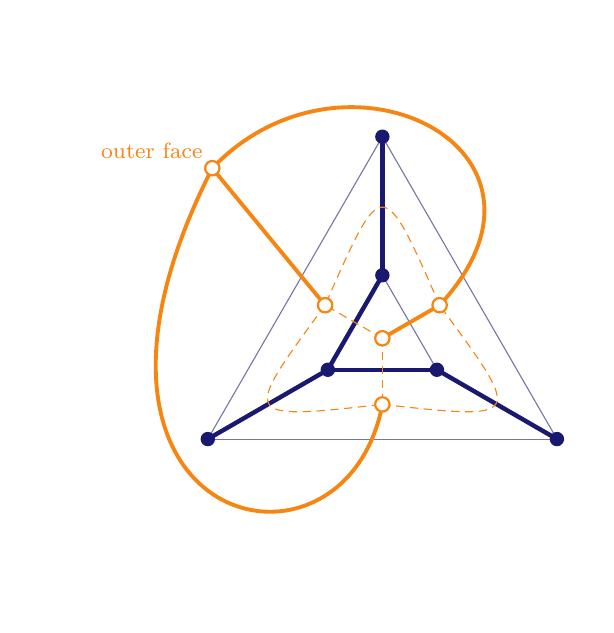
\begin{tikzpicture}[x=0.8cm,y=0.8cm,l/.style={font=\footnotesize},c/.style={font=\scriptsize,fill=white,inner sep=1pt}]
\draw[MidnightBlue,line width=1.6pt] (0.000,3.200) -- (0.000,1.000);
\draw[MidnightBlue!60] (0.000,3.200) -- (-2.771,-1.600);
\draw[MidnightBlue,line width=1.6pt] (-2.771,-1.600) -- (-0.866,-0.500);
\draw[MidnightBlue!60] (-2.771,-1.600) -- (2.771,-1.600);
\draw[MidnightBlue,line width=1.6pt] (2.771,-1.600) -- (0.866,-0.500);
\draw[MidnightBlue!60] (2.771,-1.600) -- (0.000,3.200);
\draw[MidnightBlue,line width=1.6pt] (0.000,1.000) -- (-0.866,-0.500);
\draw[MidnightBlue,line width=1.6pt] (-0.866,-0.500) -- (0.866,-0.500);
\draw[MidnightBlue!60] (0.866,-0.500) -- (0.000,1.000);
\draw[BurntOrange,densely dashed] (0.909,0.525) .. controls (0.000,2.600) .. (-0.909,0.525);
\draw[BurntOrange,densely dashed] (-0.909,0.525) .. controls (-2.252,-1.300) .. (-0.000,-1.050);
\draw[BurntOrange,densely dashed] (-0.000,-1.050) .. controls (2.252,-1.300) .. (0.909,0.525);
\draw[BurntOrange,densely dashed] (0.000,0.000) -- (-0.909,0.525);
\draw[BurntOrange,densely dashed] (0.000,0.000) -- (-0.000,-1.050);
\draw[BurntOrange,line width=1.4pt] (0.000,0.000) -- (0.909,0.525);
\draw[BurntOrange,line width=1.4pt] (-2.7,2.7) -- (-0.909,0.525);
\draw[BurntOrange,line width=1.4pt] (-2.7,2.7) .. controls (-5.6,-3.0) and (-0.6,-4.2) .. (-0.000,-1.050);
\draw[BurntOrange,line width=1.4pt] (-2.7,2.7) .. controls (-0.6,4.9) and (3.2,3.0) .. (0.909,0.525);
\fill[MidnightBlue] (0.000,3.200) circle (2.6pt);
\fill[MidnightBlue] (-2.771,-1.600) circle (2.6pt);
\fill[MidnightBlue] (2.771,-1.600) circle (2.6pt);
\fill[MidnightBlue] (0.000,1.000) circle (2.6pt);
\fill[MidnightBlue] (-0.866,-0.500) circle (2.6pt);
\fill[MidnightBlue] (0.866,-0.500) circle (2.6pt);
\filldraw[draw=BurntOrange,fill=white,thick] (-0.909,0.525) circle (2.6pt);
\filldraw[draw=BurntOrange,fill=white,thick] (-0.000,-1.050) circle (2.6pt);
\filldraw[draw=BurntOrange,fill=white,thick] (0.909,0.525) circle (2.6pt);
\filldraw[draw=BurntOrange,fill=white,thick] (0.000,0.000) circle (2.6pt);
\filldraw[draw=BurntOrange,fill=white,thick] (-2.700,2.700) circle (2.6pt);
\node[l,BurntOrange,above left] at (-2.7,2.7) {outer face};
\end{tikzpicture}
